\documentclass{beamer}

\mode<presentation>
{
  \usetheme{Frankfurt}
  \usecolortheme{orchid}
  \setbeamercovered{invisible}
  \setbeamertemplate{footline}[frame number]
}

\usepackage[english]{babel}
\usepackage[latin1]{inputenc}
\usepackage{times}
\usepackage[T1]{fontenc}
\usepackage{tikz}
\usepackage{array}
\usepackage{cancel}


\usetikzlibrary{shapes,backgrounds}

\def\multiset#1#2{\ensuremath{\left(\kern-.3em\left(\genfrac{}{}{0pt}{}{#1}{#2}\right)\kern-.3em\right)}}

\def\blue{\color{blue}~}
\def\black{\color{black}~}
\def\bl[#1]#2{\begin{block}{#1}#2\end{block}}
\def\integers{\mathbb{Z}}
\def\enumb{\begin{enumerate}}
\def\enume{\end{enumerate}}
\def\itemb{\begin{itemize}}
\def\iteme{\end{itemize}}
\def\div{~\textrm{div}~}
\def\mod{~\textrm{mod}~}


\usepackage{remreset}
\makeatletter
\@removefromreset{subsection}{section}
\makeatother
\setcounter{subsection}{1}

\title{Discrete Mathematics, Section 001, Fall 2016}
\subtitle{Lecture 17: Symmetry and Permutation}
\date{November 9, 2016}

\author[Zsolt]{Zsolt Pajor-Gyulai \\ \texttt{zsolt@cims.nyu.edu}}

\pgfdeclareimage[height=1cm]{NYUlogo}{NYUlogo.jpg}

\institute[NYU] 
{
\normalsize Courant Institute of Mathematical Sciences
}
\titlegraphic{\pgfuseimage{NYUlogo}}

\begin{document}

\begin{frame}
  \titlepage
\end{frame}

\AtBeginSection[]
{
\begin{frame}
\frametitle{Outline}
\tableofcontents[currentsection]
\end{frame}}

\section{Permutations}

\begin{frame}{Definitions}
\bl[Permutation]{Let $A$ be a set. A \textbf{permutation} on $A$ is a bijection from $A$ to itself}

For example,\vspace{-0.3cm}
\[
f=\{(1,2),(2,4),(3,1),(4,3),(5,5)\}
\]\vspace{-0.7cm}

is a permutation. In the earlier notation,\vspace{-0.2cm}
\[
f=\left[\begin{array}{ccccc}
1&2&3&4&5\\
2&4&1&3&5
\end{array}\right]
\]\vspace{-0.4cm}

\bl[]{The set of all permutations on the set $\{1,2,\dots,n\}$ is denoted by $S_n$.}
Traditional notation for permutations: $\pi,\sigma,\tau\in S_n$.
\end{frame}

\begin{frame}{The symmetric group}
\bl[]{The pair $(S_n,\circ)$ is called the \textbf{symmetric group on $n$ elements}.}
\itemb
\item The identity 
\[
\iota:=\textrm{id}_{\{1,2,\dots,n\}}
\]
is a permutation and therefore it's in $S_n$.
\item $\forall\pi,\sigma\in S_n$, $\pi\circ\sigma\in S_n$.
\item $\forall\pi,\sigma,\tau\in S_n$, $\pi\circ(\sigma\circ\tau)=(\pi\circ\sigma)\circ\tau$
\item $\forall\pi\in S_n$, $\pi\circ\iota=\iota\circ\pi=\pi$.
\item $\forall\pi\in S_n$, $\pi^{-1}\in S_n$ and $\pi\circ\pi^{-1}=\pi^{-1}\circ\pi=\iota$.
\iteme

Therefore $\circ$ is an associative operation on $S_n$ with identity $\iota$ and inverse elements being the inverses in the function sense.

\vspace{0.5cm}
Note also: $|S_n|=n!$

\end{frame}

\begin{frame}{Cycle notation}
We have seen two representations for a permutation so far, for example in $S_5$,
\[
\pi=\{(1,2),(2,4),(3,1),(4,3),(5,5)\}
\]\vspace{-0.3cm}
\[
\pi=\left[\begin{array}{ccccc}
1&2&3&4&5\\
2&4&1&3&5
\end{array}\right]
\]
Note that the top row is not necessary and we could just write $[2, 4, 1, 3, 5]$. However, for large $n$, this gets hard to decipher.
\vspace{0.5cm}

Alternatively, we can keep records of `trajectories' or \textbf{cycles}:
\[
1\quad\to\quad 2\quad \to \quad 4\quad \to\quad 3\quad\to \quad 1,\qquad\qquad 5\quad\to\quad 5
\]
and encode the information as
\[
(1,2,4,3) (5)
\]
\end{frame}

\begin{frame}{Cycle notation}
As another example, consider
\[
\pi=\left[\begin{array}{ccccccccc}
1&2&3&4&5&6&7&8&9\\
2&7&5&6&3&8&1&4&9
\end{array}\right].
\]
In the cycle notations,
\[
\pi=(1,2,7)(3,5)(4,6,8)(9)
\]

\center Practice this on Problem 1 on the Worksheet.

\end{frame}

\begin{frame}
\bl[Theorem]{Every permutation of a finite set can be expressed as a collection of pairwise disjoint cycles.}
Let $\pi\in S_n$ and consider the sequence
\[
1,\pi(1),\pi^{(2)}(1),\pi^{(3)}(1),\dots
\]
where e.g. $\pi^{(2)}(i)=(\pi\circ\pi)(i)$. 
\itemb
\item This is a sequence in $\{1,\dots, n\}$ and must repeat itself eventually.
\item Let $k$ be the first repeat, i.e
\[
\pi^{(k)}(1)\in \{1,\pi(1),\pi^{(2)}(1),\dots\pi^{(k-1)}(1)\}
\]
and $k$ is the smallest such number. FTSC assume that $\pi^{(k)}(1)\neq 1$, then
\[
\pi^{(k)}(1)=\pi^{(j)}(1)\qquad \textrm{for some }1<j<k.
\]
\iteme
[...]
\end{frame}

\begin{frame}
\bl[Theorem]{Every permutation of a finite set can be expressed as a collection of pairwise disjoint cycles.}
[...]
\itemb
\item FTSC assume that $\pi^{(k)}(1)\neq 1$, then
\[
\pi^{(k)}(1)=\pi^{(j)}(1)\qquad \textrm{for some }1<j<k.
\]
\item Because this is the first repeat, $\pi^{(k-1)}(1)\neq\pi^{(j-1)}(1)$, but then applying $\pi$ gives
\[
\pi^{(k)}(1)\neq \pi^{(j)}(1)
\]
as $\pi$ is one-to-one. $\Rightarrow\Leftarrow$
\iteme
This proves $\pi^{(k)}(1)=1$. If the cycle starting at element $1$ does not include all the elements of $\{1,2,\dots n\}$, then we can restart with an element left out and build a new cycle. That all the resulting cycles are disjoint is Problem 2 on the Worksheet.
\end{frame}

\begin{frame}
\textbf{Q:} Are there multiple cycle representations for the same permutations?
\[
\pi=\left[\begin{array}{ccccccccc}
1&2&3&4&5&6&7&8&9\\
2&7&5&6&3&8&1&4&9
\end{array}\right].
\]
\[
\pi=(1,2,7)(3,5)(4,6,8)(9)=(5,3)(6,8,4)(9)(7,1,2)
\]
However,
\itemb
\item $(1,2,7)$ and $(7,1,2)$ are the same cycles!
\item The order in which we list the disjoint cycles does not matter!
\iteme

\bl[Theorem]{Every permutation of a finite set can be expressed as a collection of pairwise disjoint cycles. \textbf{This representation is unique up to rearranging the cycles and the cyclic order of the elements within cycles.}}
\center Do Problem 3 on the Worksheet!
\end{frame}

\begin{frame}{Calculations with permutations}
\itemb
\item \textbf{Inverting:}
\[
\pi=(1,2,7,9,8)(5,6,3)(4)\in S_9
\]
Tracing it backwards:
\[
\pi^{-1}=(8,9,7,2,1)(3,6,5)(4)\in S_9
\]
\item \textbf{Compositions:}
If $\pi,\sigma\in S_9$ are
\[
\pi=(1,3,5)(4,6)(2,7,8,9),\qquad \sigma=(1,4,7,9)(2,3)(5)(6,8)
\]
Then we can read off e.g. $\pi(1)=3$ and $\sigma(3)=2$ and therefore $\sigma\circ\pi(1)=2$. Proceding similarly,
\[
\sigma\circ\pi=(1,2,9,3,5,4,8,1)(7,6)
\]
\iteme

\begin{center}
Practice this in Problem 4 on WS.
\end{center}
\end{frame}

\begin{frame}{Application to symmetries}
\begin{figure}
\centering
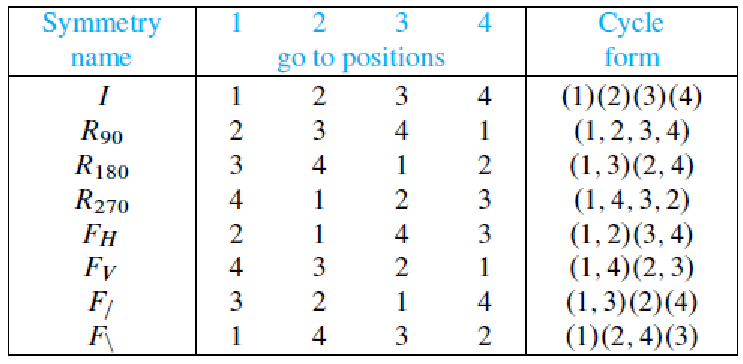
\includegraphics[scale=0.6]{aspermfull.pdf}
\end{figure}\vspace{-0.3cm}
Note that in this language, we can compute
\[
R_{90}\circ F_H~ '=' (1,2,3,4)\circ (1,2)(3,4)=(1 3)(2)(4)~'='F_/
\]
Also note that not all elements of $S_4$ are used. We call the set of symmetries of the square with the composition operation as the \textrm{dihedral group} of index $4$ and denote it by $(D_4,\circ)$.
\end{frame}

\section{Transpositions}

\begin{frame}{The simplest permutations}
The simplest possible permutation is the one that doesn't do anything:
\[
\iota=(1)(2)\dots (n)\in S_n
\]
The next symplest are called \textbf{transpositions}, which is the exchange of exactly two elements. For example,
\[
\tau=(1)(2)(3,6)(4)(5)(7)(8)(9)\in S_9
\]\vspace{-0.5cm}
\bl[Transposition]{A permutation $\tau\in S_n$ is called a \textbf{transposition} provided
\itemb
\item $\exists i,j\in\{1,2,\dots,n\}$ with $i\neq j$ so that $\tau(i)=j$ and $\tau(j)=i$,
\item $\forall k\in\{1,2,\dots,n\}$ with $k\neq i$ and $k\neq j$, we have $\tau(k)=k$.
\iteme}
Since the vast majority of cycles in a transposition are singletons, we are not going to write them and just say
\[
\tau=(3,6)
\]
\end{frame}

\begin{frame}{Writing permutations as compositions of transpositions}
\enumb
\item \textbf{Cycles:}
\[
(1,2,3,4,5)=(1,5)\circ (1,4)\circ (1,3)\circ (1,2).
\]
In general,
\[
(a_1,a_2,\dots,a_n)=(a_1,a_n)\circ (a_1,a_{n-1})\circ (a_1,a_2)
\]
\item \textbf{Any permutation:}
\begin{align*}
(1,2,&3,4,5)(6,7,8)(9)(10,11)=\\
&=[(1,5)\circ (1,4)\circ (1,3) \circ (1,2)]\circ [(6,8)\circ (6,7)]\circ (10,11)
\end{align*}
In general, put together the decomposition of the cycles.\vspace{-0.2cm}
\enume
\begin{center}
Do Problem 4 on the WS!
\end{center}
\end{frame}

\begin{frame}
\bl[Theorem]{Let $\pi$ be any permutation on a finite set. Then $\pi$ can be expressed as the composition of transpositions defined on that set.}
However, there might be other ways to do this than what our algorithm provides:
\begin{align*}
(1,2,3,4)&=(1,4)\circ(1,3)\circ (1,2)=\\
&=(1,2)\circ(2,3)\circ(3,4)=\\
&=(1,2)\circ(1,4)\circ(2,3)\circ (1,4)\circ (3,4)
\end{align*}
But note that all three versions have an odd number of transpositions!
\bl[Theorem]{Let $\pi\in S_n$. Let $\pi$ be decomposed into transpositions as \vspace{-0.3cm}
\[
\pi=\tau_1\circ\tau_2\circ\dots\circ\tau_a,\qquad \pi=\sigma_1\circ\sigma_2\circ\dots\circ\sigma_b
\]\vspace{-0.8cm}\\
Then $a$ and $b$ are either both odd or both even.}
\end{frame}

\begin{frame}{Even and odd permutations}
\bl[Theorem]{Let $\pi\in S_n$. Let $\pi$ be decomposed into transpositions as \vspace{-0.3cm}
\[
\pi=\tau_1\circ\tau_2\circ\dots\circ\tau_a,\qquad \pi=\sigma_1\circ\sigma_2\circ\dots\circ\sigma_b
\]\vspace{-0.8cm}\\
Then $a$ and $b$ are either both odd or both even.}

We are going to use the following auxiliary result:
\begin{lemma}
If the identity permutation is written as a composition of transpositions, then that composition must use an even number of transpositions. That is, if
\[
\iota=\tau_1\circ\tau_2\circ\dots\circ\tau_a,
\]
where the $\tau$-s are transpositions, then $a$ must be even.
\end{lemma}

\end{frame}

\begin{frame}
\bl[Theorem]{Let $\pi\in S_n$. Let $\pi$ be decomposed into transpositions as \vspace{-0.3cm}
\[
\pi=\tau_1\circ\tau_2\circ\dots\circ\tau_a,\qquad \pi=\sigma_1\circ\sigma_2\circ\dots\circ\sigma_b
\]\vspace{-0.8cm}\\
Then $a$ and $b$ are either both odd or both even.}

\begin{proof}
Note that we can write (HW) $\pi^{-1}$ as
\[
\pi^{-1}=\sigma_b\circ\sigma_{b-1}\circ\dots\circ\sigma_2\circ\sigma_1
\]
and thus
\[
\iota=\pi\circ\pi^{-1}=\tau_1\circ\dots\circ\tau_a\circ\sigma_b\circ\dots\circ\sigma_1.
\]
By the lemma, $a+b$ is even and so $a$ and $b$ are either both odd or both even.
\end{proof}
\end{frame}

\begin{frame}
\bl[Definition]{Let $\pi$ be a permutation on a finite set. We call $\pi$ \textbf{even} provided it can be written as the composition of an even number of transpositions. Otherwise, we call it an \textbf{odd} permutation.}

For example,
\[
(1,2,3,4)=(1,4)\circ(1,3)\circ (1,2)
\]
is an odd permutation while
\[
(1,2,3)=(1,3)\circ (1,2)
\]\vspace{-0.7cm}\\
is even.
\bl[Definition]{Let $A_n$ be the set of all even permutations in $S_n$. Then $(A_n,\circ)$ is called the alternating group.}
\end{frame}

\section{Groups}

\begin{frame}{Inverses}
\bl[Definition]{Let $*$ be an operation on a set $A$ and suppose that it has an identity element $e\in A$. Let $a\in A$. An element $b$ is an \textbf{inverse} of $a$ provided $a*b=b*a=e$.}
For example,
\begin{itemize}
\item In $(S_n,\circ)$, $(1,2,3)^{-1}=(1,3,2)$.
\item In $(\mathbb{Z},+)$, the identity element is $e=0$ and for any $a\in\mathbb{Z}$ then $(-a)+a=a+(-a)=0$ and so the inverse of $a$ is $-a$.
\end{itemize}
\textbf{Q}: Must inverses be unique?
\end{frame}

\begin{frame}{Inverses}
\bl[]{\textbf{Q}: Must inverses be unique?}
\begin{columns}
\column{0.5\textwidth}
\begin{figure}
\centering
\begin{tabular}{|c|cccc|}
\hline
*&e&a&b&c\\
\hline
e&e&a&b&c\\
a&a&a&e&e\\
b&b&e&b&e\\
c&c&e&e&c\\
\hline
\end{tabular}
\end{figure}
\column{0.5\textwidth}
\itemb
\item $e$ is an identity element.
\item $a*b=b*a=e$
\item $a*c=c*a=e$
\item Therefore $b$ and $c$ are both inverses of $a$.
\iteme
\end{columns}\vspace{0.3cm}
\itemb 
\item $(a*b)*c=e*c=c\neq a= a*e=a*(b*c)$
\item So $*$ is not associative.
\iteme


In most of our examples, the inverses were unique, but those were also associative, e.g.
\itemb
\item $(\mathbb{Z},+)$
\item $(\mathbb{Q}-\{0\},\cdot)$
\item $(S_n,\circ)$, $(A_n,\circ)$, $(D_{2n},\circ)$.
\iteme
\end{frame}

\begin{frame}{Groups}
\bl[Definition]{ Let $*$ be an operation defined on a set $G$. We call a pair $(G,*)$ a \textbf{group}, provided
\enumb
\item The set $G$ is closed under $*$; that is, $\forall g,h\in G$, $g*h\in G$.
\item $*$ is associative.
\item There is an identity $e\in G$.
\item For every element $g$, there is an inverse element $h\in G$.
\enume}

\textbf{Q}: We have seen that the identity element must be unique. Is this structure enough now for the inverse to be unique? 

\end{frame}

\begin{frame}{Uniqueness of inverses in groups}
\bl[Proposition]{Let $(G,*)$ be a group. Every element $g\in G$ has a unique inverse.}
\begin{proof}
We already know that every element has an inverse. For the sake of contradiction, assume that $g\in G$ has two (or more) distinct inverses $h,k\in G$. Then
\begin{align*}
h=h*e=h*(g*k)=(h*g)*k=e*k=k,
\end{align*}
and therefore $h=k$ giving a contradiction. $\Rightarrow\Leftarrow$
\end{proof}
Therefore we can talk about THE inverse of $g\in G$. Notation:
\itemb
\item The inverse of $g$ is mostly denoted by $g^{-1}$.
\item Sometimes for additive groups, $(-g)$ is more appropriate.
\iteme
\end{frame}

\begin{frame}{Number groups}
\itemb
\item $(\mathbb{Z},+)$: Integers with addition is a group.
\item $(\mathbb{Q},+)$: Rationals with addition is a group.
\item $(\mathbb{Q},\cdot)$: This is not a group, no $0^{-1}$.
\item $(\mathbb{Q}-\{0\},\cdot)$: This is a group.
\item $(\mathbb{Q}^+,\cdot)$: Positive rationals with multiplication is a group.
\iteme
The operation in these groups is all commutative. We have a special names for groups like this.
\bl[Definition]{We call a group $(G,*)$ \textbf{Abelian} provided $*$ is a commutative operation on $G$, i.e.
\[
g*h=h*g,\qquad\forall g,h\in G
\]}
\end{frame}

\begin{frame}{More exotic examples}
Permutation groups:
\itemb
\item $(S_n,\circ)$: permutations with composition is the \textit{symmetric group}. It is not Abelian.
\item $(A_n,\circ)$: set of all even permutations in $S_n$ is the \textit{alternating group}. (Problem 2 on WS)
\iteme
Symmetry groups:
\itemb
\item $(D_{2n},\circ)$: the symmetries of an $n$-gon is the \textit{dihedral group}.
\iteme
An odd example:
\itemb
\item If $A$ is a set $(2^A,\Delta)$ is a group (Homework).
\iteme
\end{frame}
\end{document}